\section{Introduction}
\begin{frame}{\texttt{QUESO}}
  Nutshell: \texttt{QUESO} gives samples from $\mathbb{P}(\theta | y)$ (called MCMC)
  \begin{itemize}
    \item Library for Quantifying Uncertainty in Estimation, Simulation and Optimisation
    \item Born in 2008 as part of PECOS PSAAP programme
    \item Provides robust and scalable sampling algorithms for UQ in computational models
    \item Open source
    \item \texttt{C++}
    \item \texttt{MPI} for communication
    \item Parallel chains, each chain can house several processes
    \item Dependencies are \texttt{MPI}, \texttt{Boost} and \texttt{GSL}.  Other optional features exist
    \item \textcolor{blue}{\url{http://libqueso.com}}
  \end{itemize}
\end{frame}

\begin{frame}
  \frametitle{Contributors (four \textcolor{red}{new} since v0.50.0)}
  \begin{columns}[c]
    \begin{column}{11.3cm}
      \begin{columns}[c]
        \begin{column}{5cm}
          \begin{itemize}
            \item[] \textcolor{red}{Brian Adams}
            \item[] Paul Bauman
            \item[] Morgan Bruns
            \item[] Sai Hung Cheung
            \item[] Kemelli Estacio-Hiroms
            \item[] Nicholas Malaya
            \item[] Andr\'e Maurente
            \item[] Damon McDougall
            \item[] Kenji Miki
            \item[] \textcolor{red}{Rebecca Morrison}
          \end{itemize}
        \end{column}
        %
        \begin{column}{5cm}
          \begin{itemize}
            \item[] Todd Oliver
            \item[] Sylvain Plessis
            \item[] \textcolor{red}{Teresa Portone}
            \item[] Ernesto Prudencio
            \item[] Karl Schulz
            \item[] Roy Stogner
            \item[] Gabriel Terejanu
            \item[] Rhys Ulerich
            \item[] Rochan Upadhyay
            \item[] \textcolor{red}{Eric Wright}
          \end{itemize}
        \end{column}
      \end{columns}
    \end{column}
  \end{columns}
\end{frame}

\begin{frame}{Why use QUESO?}
  Other solutions are available, e.g. R, PyMC, emcee, MICA, Stan, MUQ.
  \linebreak
  \linebreak
  QUESO solves the same problem, but:
  \begin{itemize}
    \item Has been designed to be used with large forward problems
    \item Has been used successfully with 5000+ cores
    \item Leverages parallel MCMC algorithms
    \item Supports for finite \textbf{and} infinite dimensional problems
  \end{itemize}

  \begin{figure}
    \centering
    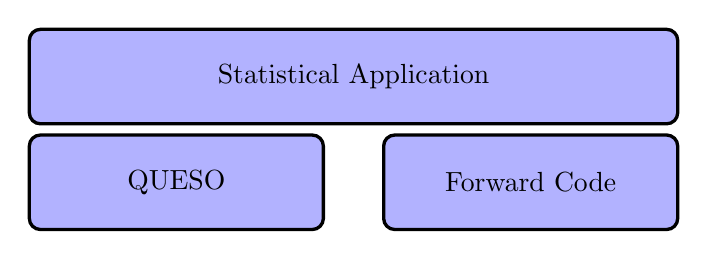
\begin{tikzpicture}[
      desc/.style={
        rectangle,
        rounded corners,
        draw=black,
        very thick,
        text centered,
        text width=8cm,
        minimum height=12mm,
        fill=blue!30
      }
    ]

    \node [desc] (StatApp) {Statistical Application};
    \node [desc, text width=3.5cm, anchor=north west, yshift=-1mm] (QUESO) at (StatApp.south west) {QUESO};
    \node [desc, text width=3.5cm, anchor=north east, yshift=-1mm] (Fwd) at (StatApp.south east) {Forward Code};

    \end{tikzpicture}
  \end{figure}
\end{frame}

\begin{frame}{Preliminaries}
  \begin{itemize}
    \item Instructions on how to build and install \Queso: \url{http://libqueso.com}
    \item All \Queso\ docs are here: \url{http://libqueso.com/queso/html/}.
    \item Links on these slides are clickable
    \item I'm British, so I spell things weird.  \Queso\ uses American English.
      \begin{itemize}
        \item It's a hard habit for me to break, so be cognizant of potential
          spelling differences in the code on these slides
        \item Try to compile stuff as we go along
      \end{itemize}
    \item These slides will not take four hours to deliver:
      \begin{itemize}
        \item There are hands-on tasks you can do.  Please do them.
        \item I encourage interruptions for questions or comments.
      \end{itemize}
    \item There are some areas of \Queso\ I am not familiar with.  I will only
      talk about the areas I am familiar with.
  \end{itemize}
\end{frame}
